% Autor: Leonhard Segger, Alexander Neuwirth
% Datum: 2017-10-30
\documentclass[
	% Papierformat
	a4paper,
	% Schriftgröße (beliebige Größen mit „fontsize=Xpt“)
	12pt,
	% Schreibt die Papiergröße korrekt ins Ausgabedokument
	pagesize,
	% Sprache für z.B. Babel
	ngerman
]{scrartcl}

% Achtung: Die Reihenfolge der Pakete kann (leider) wichtig sein!
% Insbesondere sollten (so wie hier) babel, fontenc und inputenc (in dieser
% Reihenfolge) als Erstes und hyperref und cleveref (Reihenfolge auch hier
% beachten) als Letztes geladen werden!

\usepackage{tikz}
\usetikzlibrary{calc,patterns,angles,quotes} % loads some tikz extensions\usepackage{tikz}
\usetikzlibrary{babel}

% Silbentrennung etc.; Sprache wird durch Option bei \documentclass festgelegt
\usepackage{babel}
% Verwendung der Zeichentabelle T1 (Sonderzeichen etc.)
\usepackage[T1]{fontenc}
% Legt die Zeichenkodierung der Eingabedatei fest, z.B. UTF-8
\usepackage[utf8]{inputenc}
% Schriftart
\usepackage{lmodern}
% Zusätzliche Sonderzeichen
\usepackage{textcomp}

% Mathepaket (intlimits: Grenzen über/unter Integralzeichen)
\usepackage[intlimits]{amsmath}
% Ermöglicht die Nutzung von \SI{Zahl}{Einheit} u.a.
\usepackage{siunitx}
% Zum flexiblen Einbinden von Grafiken (\includegraphics)
\usepackage{graphicx}
% Abbildungen im Fließtext
\usepackage{wrapfig}
% Abbildungen nebeneinander (subfigure, subtable)
\usepackage{subcaption}
% Funktionen für Anführungszeichen
\usepackage{csquotes}
\MakeOuterQuote{"}
% Zitieren, Bibliografie
\usepackage[sorting=none]{biblatex}


% Zur Darstellung von Webadressen
\usepackage{url}
%chemische Formeln
\usepackage[version=4]{mhchem}
% siunitx: Deutsche Ausgabe, Messfehler getrennt mit ± ausgeben
\usepackage{floatrow}
\floatsetup[table]{capposition=top}
\usepackage{float}
% Verlinkt Textstellen im PDF-Dokument
\usepackage[unicode]{hyperref}
% "Schlaue" Referenzen (nach hyperref laden!)
\usepackage{cleveref}
\sisetup{
	locale=DE,
	separate-uncertainty
}
\bibliography{BA-C-04_V05_08-04-2019_References}

\begin{document}

	\begin{titlepage}
		\centering
		{\scshape\LARGE Versuchsbericht zu \par}
		\vspace{1cm}
		{\scshape\huge V05 - Lebensdauermessung eines $\gamma$-Niveaus \par}
		\vspace{2.5cm}
		{\LARGE Gruppe BA-C-04 \par}
		\vspace{0.5cm}

		{\large Alexander Neuwirth (E-Mail: a\_neuw01@wwu.de) \par}
		{\large Leonhard Segger (E-Mail: l\_segg03@uni-muenster.de) \par}
		\vfill

		durchgeführt am 08.04.2019\par
		betreut von\par
		{\large Raffaela Busse} \par %TODO Ich würde die hier legit rausnehmen. Die hat halt offiziell nur zugeschaut (und auch faktisch)
		und \par
		{\large Daniel Guderian}
		\vfill

		{\large \today\par}
	\end{titlepage}
	\tableofcontents
	\newpage

	%TODO mehr TODO in Default

	\section{Kurzfassung}
	% Hypothese	und deren Ergebnis, wenn Hypothese ist, dass nur Theorie erfüllt, sagen: Erwartung: Theorie aus einführung (mit reflink) erfüllt
	% Ergebnisse, auch Zahlen, mindestens wenn's halbwegs Sinn ergibt
	% Was wurde gemacht
	% manche leute wollen Passiv oder "man", manche nicht
	In diesem Versuch wird die mittlere Lebensdauer des ersten angeregten $\gamma$-Niveaus in Scandium-44 gemessen.
	Dazu wird verwendet, dass Titan-44 nach dem Zerfall durch Elektroneneinfang in einen angeregten Zustand von Scandium-44 übergeht.
	Dieser Zustand wird dann zunächst durch Aussenden eines Photons zum untersuchten Zustand, der dann unter erneutem Aussenden eines Photons in den Grundzustand übergeht.
	Deshalb wird die Zeitdifferenz zwischen den ausgesandten Photonen über viele Ereignisse gemessen und dann über Bestimmung des Mittelwerts, Fit mit einer Exponentialfunktion und Bestimmung der Halbwertsbreite die mittlere Lebensdauer des untersuchten Niveaus bestimmt.
	Dazu muss zunächst durch zusätzliche Messungen der Versuchsaufbau kalibriert werden.
	Hierzu wird das beim Beta-Zerfall des Scandiums entstehende Positronium genutzt.

  \section{Theorie}
	% wdh. Texte
	% wdh. Besprechung
	\subsection{Zerfall von Titan-44}

	Das Zerfallsschema von Titan-44 ist in \cref{fig_Zerfallsschema} dargestellt. Titan-44 zerfällt über Elektroneneinfang mit einer Halbwertszeit von \SI{2,44}{} Tagen zu einem angeregten Niveau von Scandium-44 (\cite{Anleitung}).
	Das angeregte Scandium-44 sendet dann zwei $\gamma$-Photonen beim Abregen auf das zu untersuchende mittlere Niveau und dann in den Grundzustand aus.
	%Hierbei ist zu erwähnen, dass die erste Abregung mit einer Halbwertszeit von \SI{0,15}{\mikro \seconds} stattfindet %nvm schätze das ist doch egal. %TODO oder muss man hier wissen, dass das nicht lange in dem oberen Niveau ist, wir hatten irgendwas bei der Vorbesprechung gesagt, aber war glaube ich halbgar
	Der Grundzustand von Scandium-44 zerfällt dann durch Beta-Plus-Zerfall in einen angeregten Zustand von Calcium-44, der dann wiederum durch Aussenden eines $\gamma$-Photons in den Grundzustand über.
	Für die Versuchsdurchführung sind die beiden Photonen bei der Abregung des Scandiums und der Beta-Plus-Zerfall relevant.

	\begin{figure}[H]
			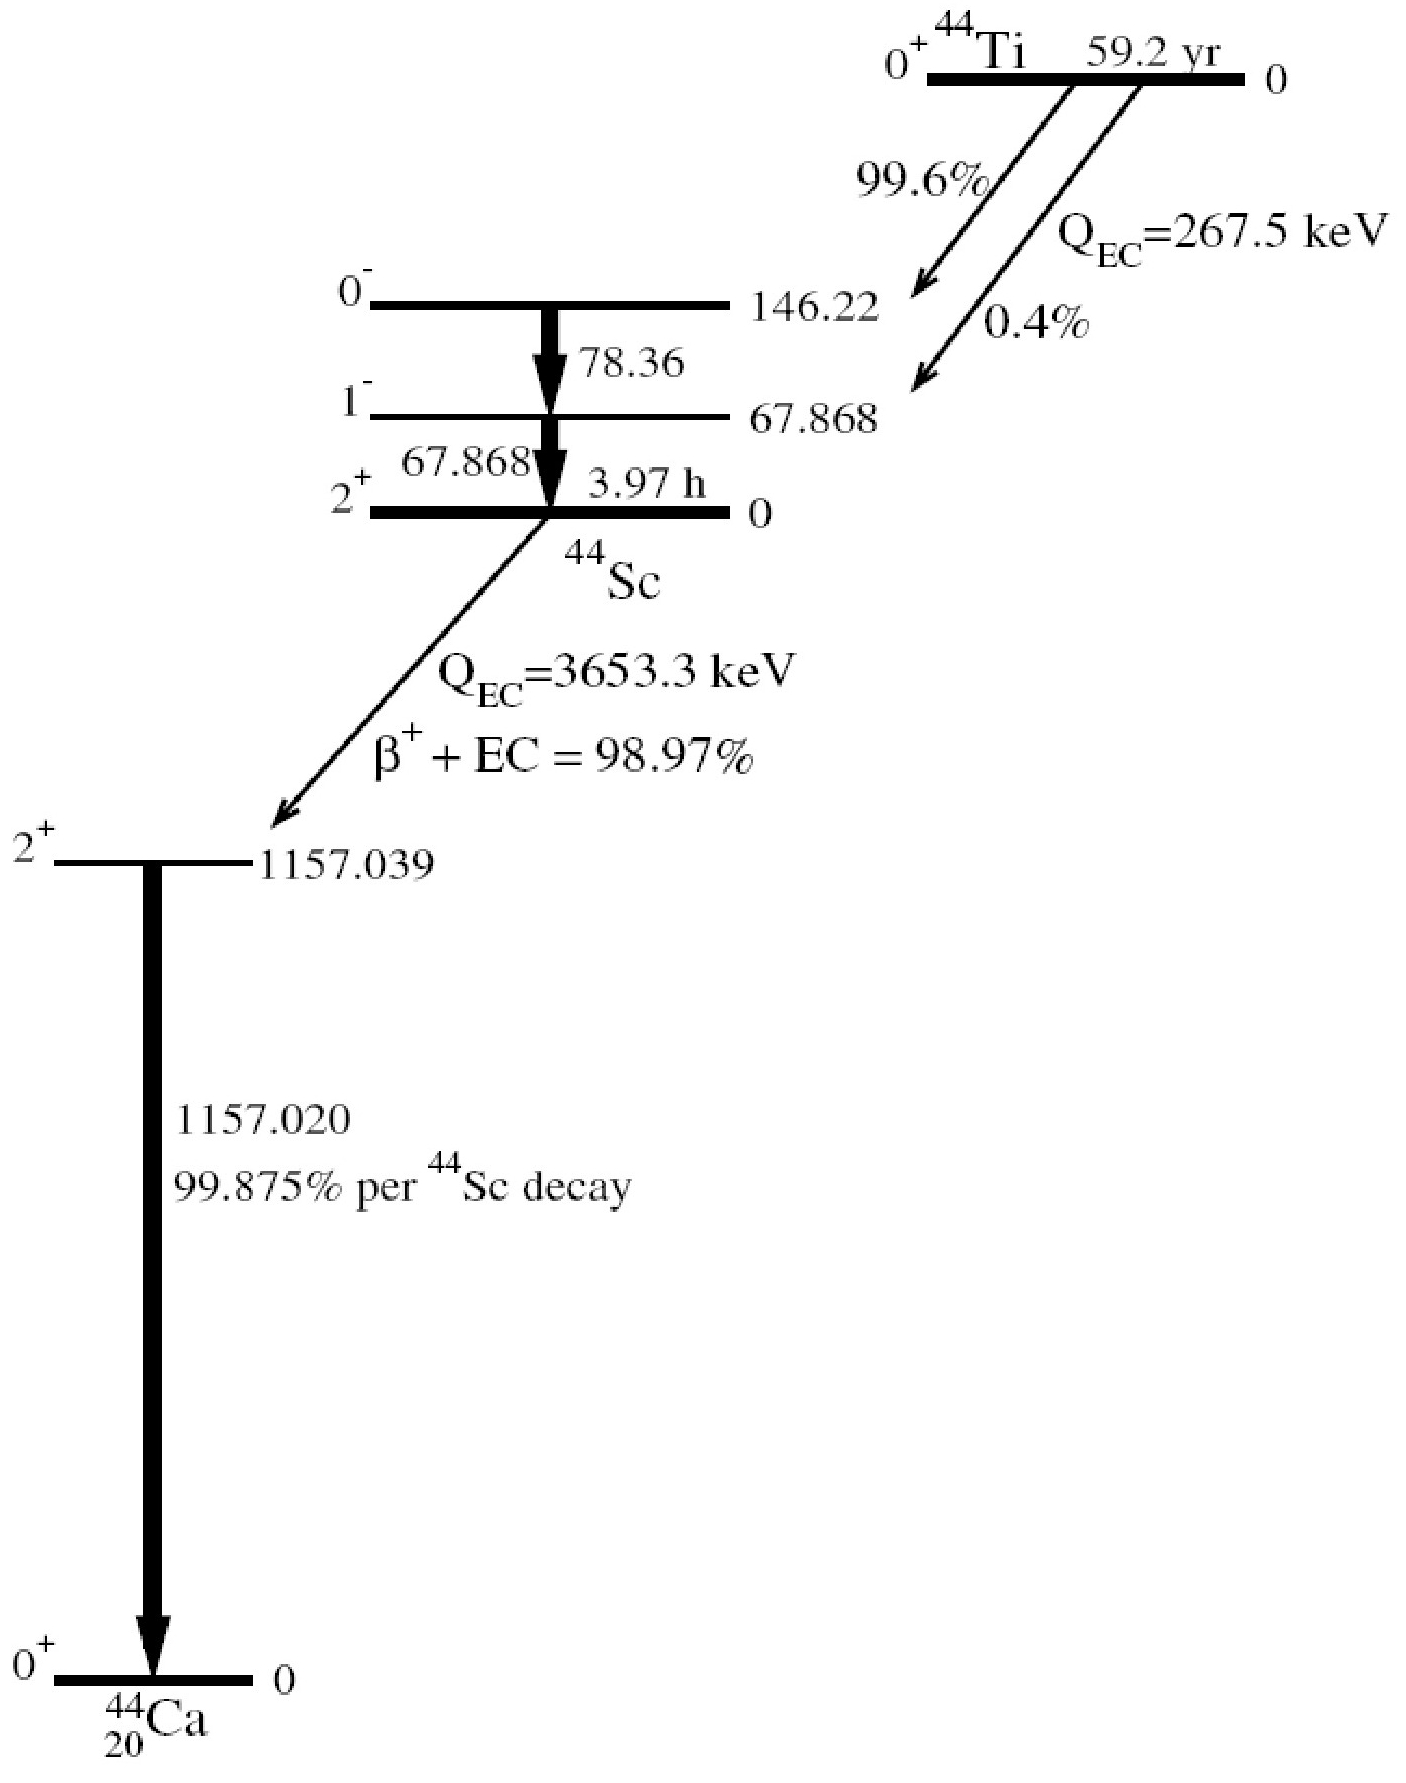
\includegraphics[width=0.6\linewidth]{img/44Ti-decay_reduziert}
			\caption{
			Reduziertes Zerfallsschema von Titan-44 über Scandium-44 zu Calcium-44. Zerfallswege geringer Wahrscheinlichkeit sind nicht dargestellt.
			\cite{Zerfallsschema} %TODO theoretisch copyrightmäßig schwierig, weil ich den unnötigen Teil rausgecropt habe. Alternative: Anleitung scannen.
			}
			\label{fig_Zerfallsschema}
	\end{figure}

	%TODO mehr zu gamma-abregung?
	\subsection{Elektroneneinfang}
	%TODO Elektroneneinfang erklären bzw Gleichung hinschreiben!
	\subsubsection{Beta-Plus-Zerfall}
	Wie oben beschrieben findet die folgende Kernreaktion statt:
	\begin{equation}
		\label{eq_beta-plus}
		 _{21}^{44}\text{Sc} \rightarrow _{20}^{44}\text{Ca} + \text{e}^+ + \nu_{\text{e}}
	\end{equation}
	Das dabei entstandene Positron wird durch Wechselwirkung mit dem Rest der Probe abgebremst.
	Wenn es ausreichend stark abgebremst ist, kann es mit einem Elektron in der Probe das instabile Positronium bilden.
	Beim Positronium unterscheidet man je nach Spinausrichtung von Positron und Elektron in Parapositronium ($S=0$) und Orthopositronium ($S=1$).
	Aufgrund von Spin- und Impulserhaltung zerfällt Orthopositronium in eine ungerade Anzahl Photonen, die mindestens \num{3} beträgt.
	Aus analogen Gründen zerfällt Parapositronium eine gerade Anzahl Photonen, aber mindestens \num{2}.
	Da Zerfälle, die die Produktion einer geringeren Menge an Photonen voraussetzt, wahrscheinlicher sind, zerfällt Orthopositronium deutlich langsamer als Parapositronium.
	Gleichzeitig kann durch Umgebungswechselwirkung Orthopositronium in Parapositronium übergehen, was während der vergleichsweise langen Zerfallsdauer wahrscheinlich ist.
	Deswegen kann man sich in den folgenden Betrachtungen im Wesentlichen auf den Zerfall von Parapositronium in zwei Photonen mit einer Energie von \SI{511}{keV} beschränken.
	Außerdem ist anzumerken, dass die mittlere Lebensdauer von Parapositronium bei \SI{125}{ps} liegt, was im Vergleich zur erwarteten Lebensdauer des untersuchten $\gamma$-Niveaus verschwindend gering ist (\cite{Anleitung}).

	\subsection{Wechselwirkung der $\gamma$-Photonen mit Materie}

	Die bei den zuvor beschriebenen Zerfallsprozessen entstandenen Photonen können mit Kern oder Hüllenelektronen der Umgebung oder deren elektromagnetischen Feldern wechselwirken.
	Da die Wechselwirkung mit Atomkernen aufgrund des geringen Anteils des Kernvolumens am Atomvolumen einen deutlich geringeren Wirkungsquerschnitt hat, überwiegt die Wechselwirkung mit Hüllenelektronen.

	\subsubsection{Photoeffekt}
	Ein einfallendes $\gamma$-Photon kann im Atom absorbiert werden und die Emission eines Hüllenelektrons aus dem Atom heraus zufolge haben.
	Das herausgelöste Elektron erhält dabei die Differenz zwischen Energie des einfallenden Photons und der nötigen Ionisierungsenergie, um es aus dem Atom zu lösen.
	Auf das nun unbesetzte Energieniveau kann ein Elektron aus einer höheren Schale (oder ein freies Elektron) absinken, wobei ein Photon charakteristischer Energie (bei freien Elektronen kontinuierliches Spektrum ab einer Mindestenergie) frei wird. % das freie Elektron ist halt unwahrscheinlich, aber ich habs mal trotzdem erwähnt.

	\subsubsection{Compton-Effekt}
	Bei der Compton-Streuung überlebt im Gegensatz zum Photoeffekt das einfallende $\gamma$-Photon und bewegt sich danach im Allgemeinen mit geänderter Richtung und Energie.
	Wenn die Energie des einfallenden Photons deutlich größer als die Ionisierungsenergie ist, kann das Hüllenelektron wie ein freies Elektron betrachtet werden.
	Die Energieänderung des Photons hängt dann nur vom Winkel der Richtungsänderung und seiner Ursprungsenergie ab.

	\subsubsection{Paarbildungseffekt}

	Hier wird im Coulomb-Feld eines Atomkerns ein $\gamma$-Photon in ein Positron und eine Elektron umgewandelt.
	Dies kann aufgrund von Energie- und Impulserhaltungssatz nur in Wechselwirkung mit einem Atomkern stattfinden.

	\subsection{Szintillator}

	Ein Szintillator ist ein Detektor, der einfallende Strahlung in eine einfacher messbare elektromagnetische Strahlung umwandelt.
	In diesem Versuch wurde ein anorganischer Halbleiter-Szintillator verwendet.
	Bei diesem wird durch die einfallende Strahlung ein Elektron aus den Valenzband in das Leitungsband angeregt und lässt im Valenzband ein Loch zurück.
	Wenn das Elektron an einer Störstelle mit dem Loch rekombiniert, kann dies durch die an der Störstelle modifizierten Bandstruktur schrittweise geschehen, weshalb Strahlung einer geringeren, leichter detektierbaren Wellenlänge frei wird.

	\subsection{Photomultiplier}

	In einem Photomultiplier werden einzelne einfallende Photonen in ein messbares Signal umgewandelt.
	Das Funktionsprinzip ist in \cref{fig_Photomultiplier} dargestellt.
	Dabei löst zunächst ein einfallendes Photon an der Kathode (negative Spannung) ein Elektron aus.
	Dieses Elektron wird in Richtung der Anode (positive Spannung) beschleunigt und schlägt auf dem Weg dorthin aus den Dynoden zusätzliche Elektronen heraus.
	An der Anode kommen dann ausreichend viele Elektronen an, um einen messbaren Rückfluss zur Kathode zu erzeugen (bzw. über einen Widerstand eine messbare Spannung).

	\begin{figure}[H]
			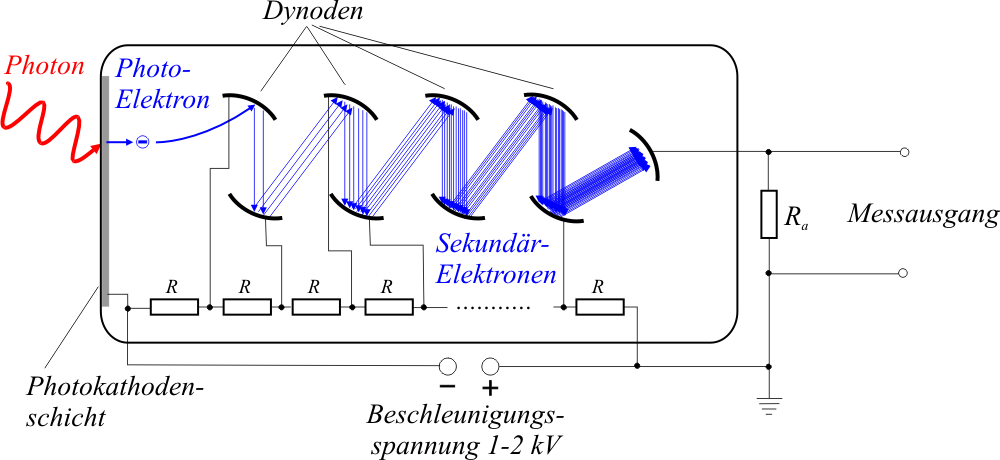
\includegraphics[width=0.6\linewidth]{img/Photomultiplier}
			\caption{
			Schematische Darstellung eines Photomultipliers.
			\cite{Photomultiplier}
			}
			\label{fig_Photomultiplier}
	\end{figure}

	\section{Methoden}
	% Bilder von der Website klauen
	% einer will Präsens
	%TODO Detektionsmechanismus
	%TODO welche Geräte haben welche Funktion
	Der Versuch wird in zwei Teilen durchgeführt und eine Titan-44-Probe untersucht.
	Zunächst wird der Zerfall des nach dem Beta-Zerfall entstehenden Positroniums genutzt, um eine Zeitkalibrierung zu ermöglichen.
	Dann wird die Zeitdifferenz der $\gamma$-Photonen der schrittweisen Abregung von Scandium-44 genutzt, um die Lebensdauer des mittleren Niveaus zu bestimmen.

	%Die eine Titan-44-Probe verlassende $\gamma$-Strahlung soll detektiert werden.
	%Zusätzlich soll die zeitliche Differenz zwischen zwei $\gamma$-Photonen eines bestimmten Energiefensters gemessen werden.

	Verwendet werden zwei Detektoren, die Szintillator und Photomultiplier kombinieren, um ein Signal zu erzeugen, das proportional zum einfallenden Photon ist.
	Diese werden mit Hochspannung (\SI{1400}{V} und \SI{1100}{V}) betrieben.
	Die Signale werden zunächst vorverstärkt und dann in einen Spektralverstärker geleitet.
	Dieser verstärkt das Signal einerseits zusätzlich und wandelt es in eine Form um, die später bei der Ermittlung der Zeitdifferenz Effekte von Walk und Jitter minimiert.
	Hierbei wird statt dem Überschreiten eines bestimmten Schwellenwerts der Nulldurchgang des näherungsweise sinusförmigen (eine Periode) Signals verwendet als zu vergleichender Zeitpunkt verwendet.

	\subsection{Energiefilterung}

	Die Detektoren werden im \SI{180}{\degree}-Winkel zueinander auf die Probe gerichtet.
	Mit dem Aufbau bis zu diesem Punkt wird nun die Energie der Signale mit einem Multi Channel Analyzer in Kanäle aufgeteilt, digitalisiert und über einen Zeitraum von wenigen Minuten gemessen. %TODO ich bin mir nicht sicher, ob für das Energiegedöns das Signal schon umgeformt wurde...
	Die gemessenen Ereignisse werden dann über die entsprechenden Kanäle aufgetragen.
	In dem so gemessenen Energiespektrum wird der zum Zerfall des Positroniums gehörige Peak (\SI{511}{keV}) und der zur Abregung von Scandium-44 gehörige Peak (\SI{87,4}{keV} und \SI{67,8}{keV}) identifiziert und Anfang und Ende des Peaks im Kanalspektrum notiert.
	Über einen Dreisatz wird aus den Gesamtkanälen (8192) und dem möglichen Spannungsintervall (\SIrange{0}{10}{\volt}) der Signale der Spannungsbereich berechnet, in dem die Signale der Abregung und des Positroniumzerfalls liegen.
	Dies wird für beide Detektoren getrennt durchgeführt.

	\subsection{Zeitkalibrierung}
	Für diesen Versuchsteil der untersuchte Bereich auf den zum Positronium gehörigen Spannungsbereich begrenzt.
  Die übrigen Signale werden dann in einen Timing Single Channel Analyzer in ein Rechtecksignal konvertiert, wobei der Nulldurchgang für den Beginn des Rechtecksignals genutzt wird.
	Die Rechtecksignale von beiden Detektoren werden dann in einem Time to Amplitude Converter geleitet, der die zeitliche Differenz zwischen den Rechtecksignalen der beiden Detektoren in Ausgangssignal umwandelt, dessen Höhe proportional zur Zeitdifferenz ist.
	Dieses Signal wird dann vom Multichannel Analyzer digitalisiert und in Kanäle in Abhängigkeit von der Signalhöhe getrennt.
	Da die beiden Photonen vom Positronium im \SI{180}{\degree}-Winkel zeitgleich emittiert werden, kann nun der Zeitnullpunkt ermittelt werden, da hier das Maximum der gemessenen Ereignisse liegt.
	Die Zeitdifferenz aufgrund der Postion des Positroniums in der Probe wird hierbei vernachlässigt, da sie aufgrund der Bewegung der Photonen mit Lichtgeschwindigkeit verschwindend gering ist.

	Nun muss noch die Kanalbreite in eine Zeitdifferenz umgerechnet werden können.
	Hierfür wird anstelle der Detektoren ein Signalgenerator verwendet, der im Abstand vom \SI{640}{\nano \second} Signale erzeugt.
	Diese werden im Kanalspektrum aufgetragen und auf Basis des Mittelwerts der Abstände der Signale der Umrechnungsfaktor von Kanalbreite und Zeitdifferenz bestimmt.

	\subsection{Messung der mittleren Lebensdauer}

	Die Detektoren werden nun im \SI{90}{\degree}-Winkel zueinander auf die Probe gerichtet, um die Messung von Positronium auszuschließen und zusätzlich der Spannungsbereich nach dem Spektralverstärker auf den Bereich der Abregung von Scandium-44 begrenzt.
	Dann werden über \num{25} Stunden die auftretenden Ereignisse gemessen.
	Da diese die zeitlichen Differenzen zwischen Aussendung des Photons bei Abregung auf den mittleren angeregten Zustand und Abregung auf den Grundzustand darstellen, kann so die mittlere Lebensdauer des mittleren angeregten Zustands bestimmt werden.
	%  Zeiten
	% Zeitdifferenz: 25.3h
	% Positronium_Zeitdifferenz: 1.2h
	% Zeitkalibrierung: 7s
	% Energy_Start: 3.7m
	% Energy_Stop: 11.4m


	\section{Ergebnisse und Diskussion}
	%TODO Unsicherheiten


	\subsection{Beobachtung und Datenanalyse}
	% Allgemeine Beobachtungen
	% Einflüsse von veränderten Parametern auf Messung
	\subsubsection{Unsicherheiten}
	% Berechung nach Aufgabenstellung

	\subsection{Energiespektren}
	Zuächst wurden die Energeispektren \cref{fig_energy_start} und \cref{fig_energy_stop} gemessen. Hieraus wurden die Kanalbereiche für aus dem jeweiligen Prozess stammende Photonen ermittelt.

	%TODO Peaks der zwei Zerfälle nicht unterscheidbar

	\begin{figure}[H]
				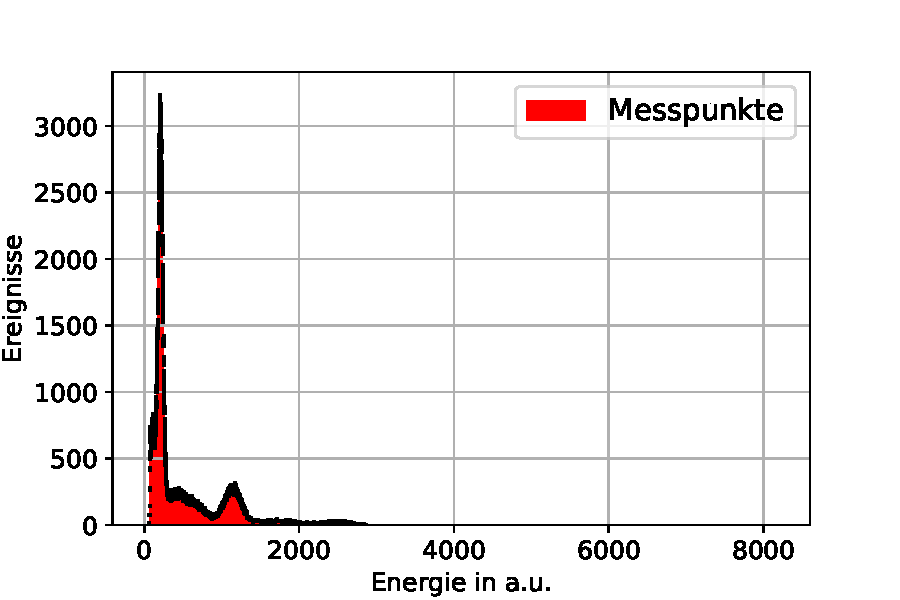
\includegraphics[width= 0.9 \linewidth]{img/Energiespektrum_Start}
				\caption{
				Energiespektrum welches von der ersten Messapparatur aufgenommen wurde.
				Die Energie ist in willkürlichen Einheiten angegeben, da nicht bekannt ist, welcher Photonenenergie der Multi Channel Analyzer welchen Kanal zuordnet, aber bekannt ist, dass ein höherer Kanal auch einer höheren Energie entspricht.
				Die Unsicherheiten sind in Schwarz abgebildet, sodass sich der Messwert mittig im schwarzen Bereich befindet.
				}
				\label{fig_energy_start}
		\end{figure}

	\begin{figure}[H]
				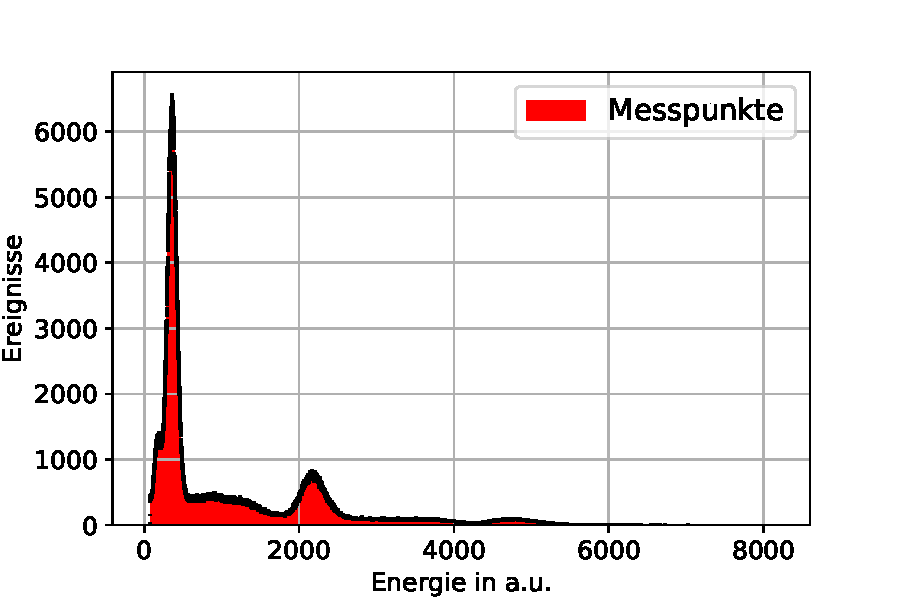
\includegraphics[width= 0.9 \linewidth]{img/Energiespektrum_Stop}
				\caption{
				Energiespektrum welches von der zweiten Messapparatur aufgenommen wurde.
				Die Energie ist in willkürlichen Einheiten angegeben, da nicht bekannt ist, welcher Photonenenergie der Multi Channel Analyzer welchen Kanal zuordnet, aber bekannt ist, dass ein höherer Kanal auch einer höheren Energie entspricht.
				Die Unsicherheiten sind in Schwarz abgebildet, sodass sich der Messwert mittig im schwarzen Bereich befindet.
				}
				\label{fig_energy_stop}
		\end{figure}

  \subsubsection{Zeitkalibrierung}
	Der Mittelwert der Abstände der Peaks in \cref{fig_zeitkalibrierung} beträgt \SI{514.8+-0.4}{}, das heißt, so viele Kanäle entsprechen einer Zeit von \SI{0.64+-0.003}{\mu s}.

	\begin{figure}[H]
				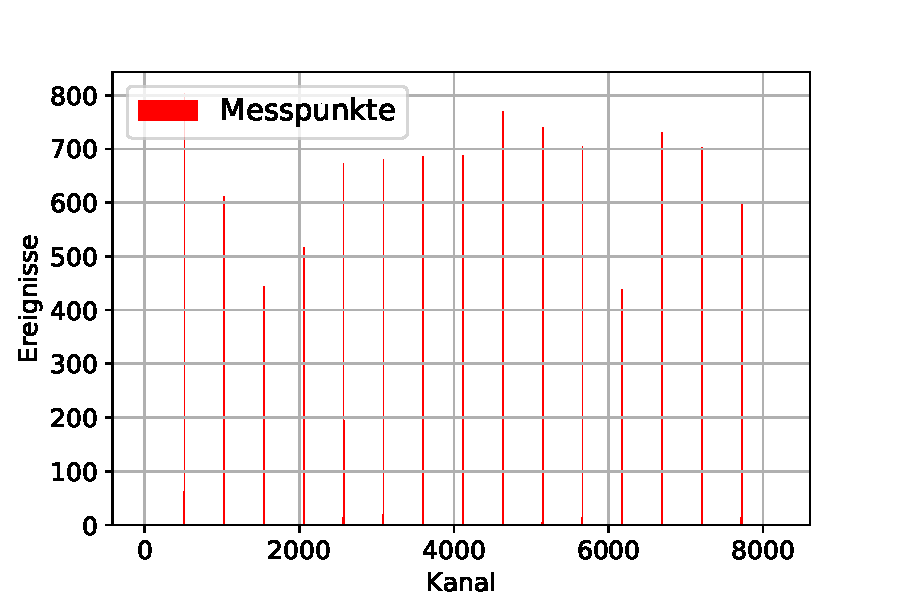
\includegraphics[width= 0.9 \linewidth]{img/Zeitkalibrierung}
				\caption{
				Zeitkalibrierung der Kanäle mittels eines Signalgenerators.
				Es gibt auch kleine Beiträge zu anderen Kanälen in naher Umgebung der Peaks, jedoch sind diese aufgrund der zu geringen Auflösung des Bildes kaum sichtbar.
				}
				\label{fig_zeitkalibrierung}
		\end{figure}

		\subsubsection{Bestimmung des Nullpunkts}
		In \cref{fig_positronium_zeitdifferenzen} sind die Messungen der Zeitdifferenzen des Positroniumzerfalls abgebildet.
		Da dieser sehr scharf ist, ist er in \cref{fig_positronium_zeitdifferenzen_zoom} vergrößert dargestellt.
		Es wird eine Gaußfunktion \ref{eq_gauss} an die Messpunkte angepasst.
		\begin{equation}
			\label{eq_gauss}
			%A * np.exp(-(x - x0)**2 / 2 / d**2)
			 f(t) = N\exp\left\{{\frac{(t-T_0)^2}{2 \Delta T^2}}\right\}
		\end{equation}
		Die Standardabweichung des Fits $\Delta T$ beschreibt für die folgende Bestimmung der Lebensdauer des $\gamma$-Niveaus die Unsicherheit der Messapparatur bei der Auflösung von Zeitdifferenzen, da beim Positroniumzerfall kein zeitlicher Unterschied vorliegt. %TODO ref in Theorie? bzw. vernachlässigbar klein

	\begin{figure}[H]
				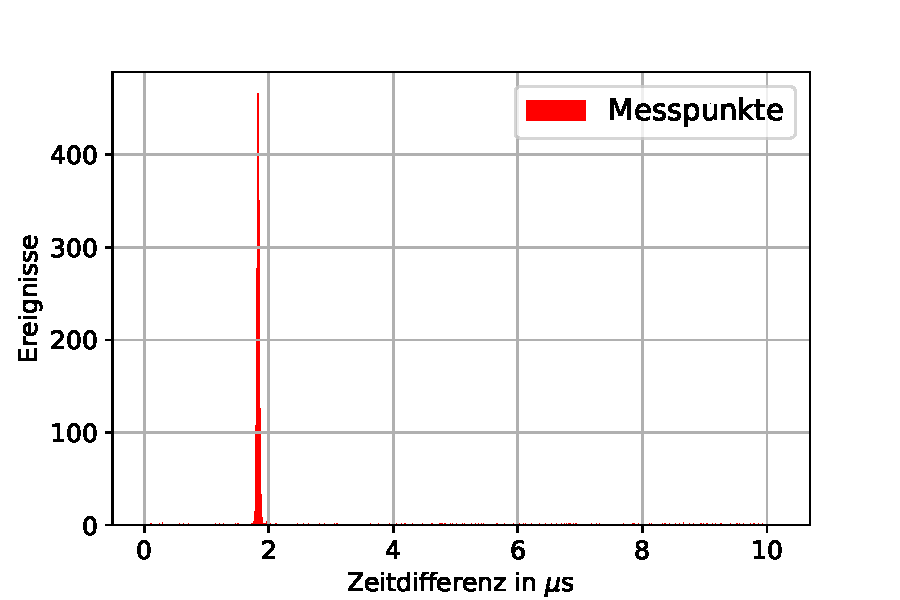
\includegraphics[width= 0.9 \linewidth]{img/Positronium_Zeitdifferenz}
				\caption{
				Zeitdifferenz zwischen den Photonen des Positroniumzerfalls.
				Die Unsicherheiten sind in Schwarz abgebildet, sodass sich der Messwert mittig im schwarzen Bereich befindet.
				}
				\label{fig_positronium_zeitdifferenzen}
		\end{figure}

	\begin{figure}[H]
				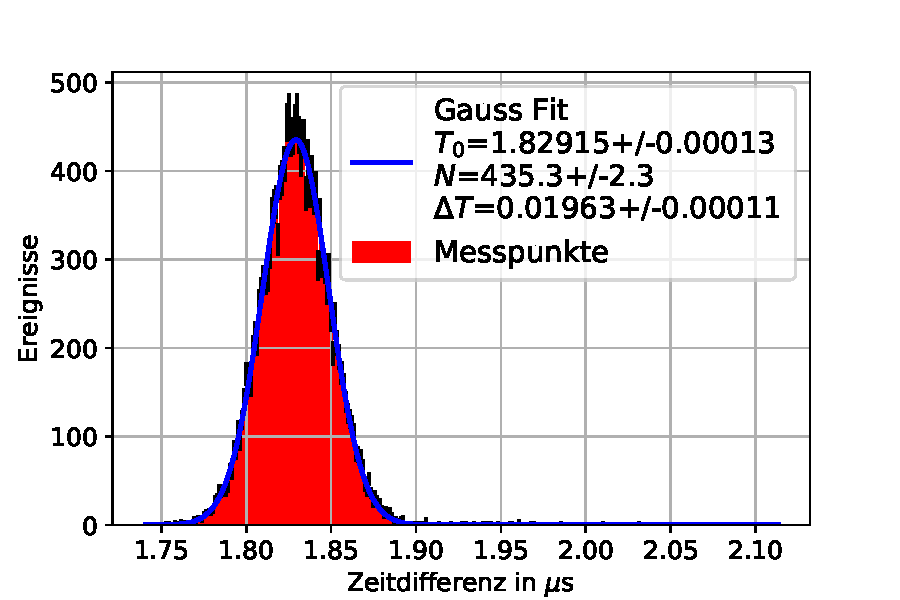
\includegraphics[width= 0.9 \linewidth]{img/Positronium_Zeitdifferenz_zoom}
				\caption{
				Zeitdifferenz zwischen den Photonen des Positroniumzerfalls.
				Die Unsicherheiten sind in Schwarz abgebildet, sodass sich der Messwert mittig im schwarzen Bereich befindet.
				}
				\label{fig_positronium_zeitdifferenzen_zoom}
		\end{figure}

		\subsubsection{Bestimmung der Lebensdauer}

		\subsubsection*{Abschätzung}
		Mit \cref{fig_zeitdifferenz_zoom} wurde die Halbwertszeit grob abgeschätzt.
		Hierbei beschreibt die grüne Horizontale bei \SI{125}{} Ereignissen den Untergrund (siehe \cref{fig_zeitdifferenz}).
		In gelb verlaufen eine Horizontale und eine Vertikale durch das abgeschätzte Maximum.
		Ebenso ist der Punkt der mit halb so vielen Ereignissen (ohne den Untergrund) lila markiert.
		Die Differenz gibt die Halbwertszeit $t_{1/2}=\SI{150+-50}{ns}$.
		\begin{figure}[H]
				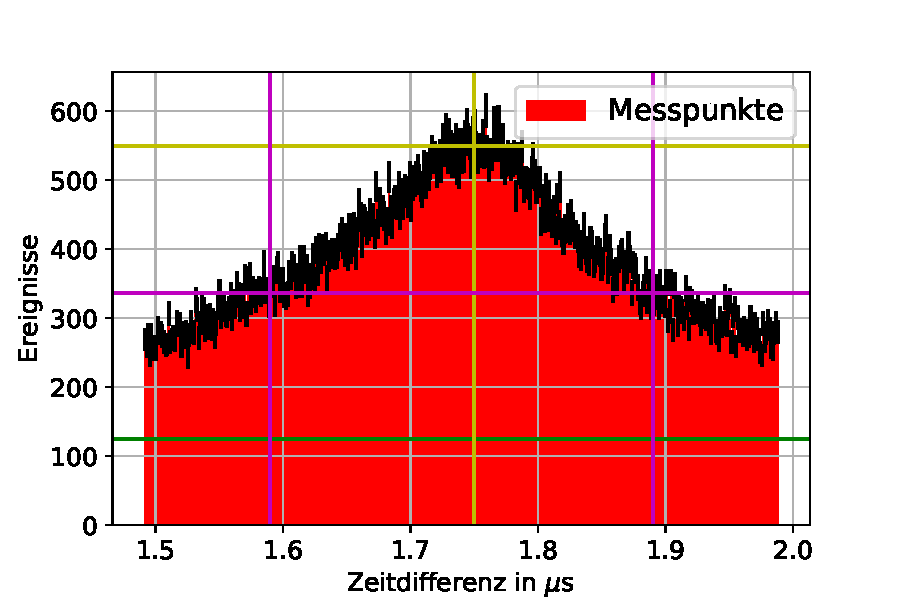
\includegraphics[width= 0.9 \linewidth]{img/Zeitdifferenzen_zoom}
				\caption{
					$\gamma$-Niveau-Kanal:
				Die Unsicherheiten sind in Schwarz abgebildet, sodass sich der Messwert mittig im schwarzen Bereich befindet.
				}
				\label{fig_zeitdifferenz_zoom}
		\end{figure}
		\subsubsection*{Fit}
		In \cref{fig_zeitdifferenz} ist die Grüne Linie der Mittelwert aller Ereignisse bei einer Zeitdifferenz größer \SI{4}{\mu s}.
		Der lila Fit ist in in die jeweilige Richtung ein exponentiell abfallende Funktion:
		\begin{equation}
			\label{eq_dexp}
			f(t)=N\cdot (\exp{-\left\{\lambda_1(t-T_0)\right\}}\Theta(t-T_0)+\exp{\left\{\lambda_2(t-T_0)\right\}}\Theta(T_0-t))
		\end{equation}
	\begin{figure}[H]
				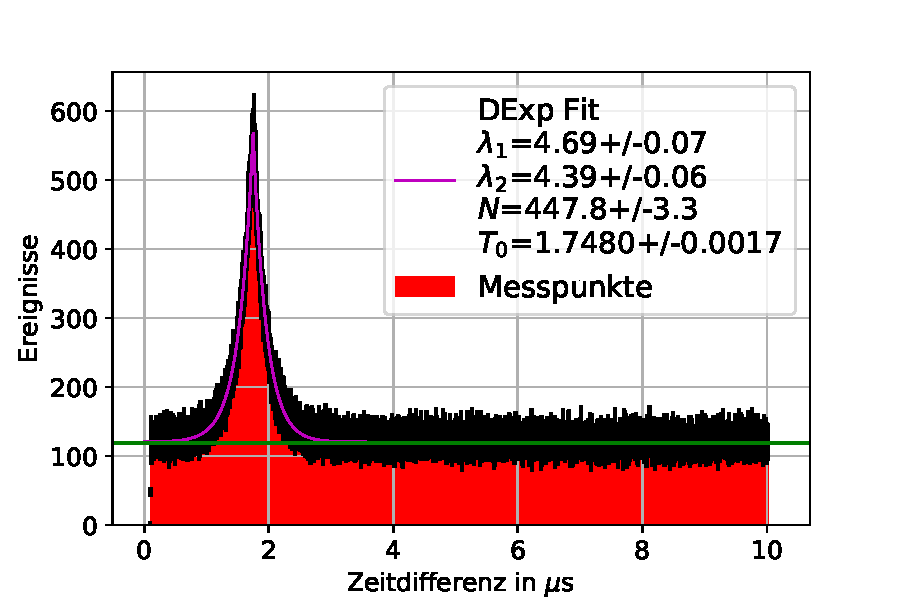
\includegraphics[width= 0.9 \linewidth]{img/Zeitdifferenzen}
				\caption{
					$\gamma$-Niveau-Kanal:
				Die Unsicherheiten sind in Schwarz abgebildet, sodass sich der Messwert mittig im schwarzen Bereich befindet.
				}
				\label{fig_zeitdifferenz}
		\end{figure}
		\subsubsection*{Integration}

		In \cref{tb_leb} sind die insgesamt resultierenden Lebensdauern aufgeführt.
		\begin{table}[H]
		\centering
		\begin{tabular}{c | c | c | c  }
			 Index&$\lambda$ in \si{\mu s^{-1}}& $\tau=1/\lambda$ in \si{ns} &$t_{1/2}=\tau\ln 2$ in \si{ns}\\ \hline
			 1&\SI{4.68+-0.07}{}&\SI{213+-3}{}&\SI{147+-2}{} \\
			 2&\SI{4.39+-0.06}{}&\SI{228+-3}{}&\SI{158+-2}{} \\
			 3\\
			 4\\
		\end{tabular}
		\caption{
		Verschiedene gemessene Lebensdauern, bzw. Halbwertszeiten, des angeregten $\gamma$-Niveaus von $^{44}$Sc.
		}
			 \label{tb_leb}
	\end{table}
	\subsection{Diskussion}
	% Bezug/Nutzen oder sonst was
	% auch hier die Hypothese wiederholen
	% keine Messwerte hier, nach manchen Menschen, zumindest "direkt" erstellte Diagramme net hier, auch wenn Lesbarkeit-bla
	In den Energiespektren in \crefrange{fig_energy_start}{fig_energy_stop} wird dem höchsten Peak die Photonen aus der Abregung von Scandium-44 zugeordnet.
	Diese sind aufgrund des geringen Energieunterschieds von \SI{11}{keV} nicht unterscheidbar.
	Dem deutlich kleineren, aber immer noch ausgeprägten Peak bei höherer Energie werden die Photonen des Positroniumzerfalls bei \SI{511}{keV} zugeordnet.
	Die Bestimmung des Zeitnullpunkt aus der Messung mittels Signalgenerators (\cref{fig_positronium_zeitdifferenzen_zoom}) ist möglich, liefert aber ein anderes Ergebnis, als die aus der Position des Maximums der Zeitdifferenzen bei der Scandium-44-Abregung (\cref{fig_zeitdifferenz}).
	Eine Erklärung für diesen Effekt bleiben wir hier schuldig, da sich lediglich die Ausrichtung der Detektoren geändert hat.

	%TODO Vergleich der verschiedenen mittleren Lebensdauern mit Literaturwert
	Literaturwert liegt bei \SI{}{} (\cite{})

	\subsubsection{Vergleich der Ergebnisse}

	%TODO unterschiedlicher Zeitnullpunkt
	\section{Schlussfolgerung}
	% Rückgriff auf Hypothese und drittes Nennen dieser
	Insgesamt gesehen lässt sich sagen, dass die Lebensdauer des untersuchten ersten angeregten $\gamma$-Niveaus in Scandium-44 erfolgreich bestimmt werden konnte.
	%TODO Ergebnis Vergleich der Varianten
	%TODO Vergleich Literaturwert
	Nicht geklärt werden konnte, warum bei der Messung von Positronium-Photonen und Scandium-Photonen unterschiedliche Zeitdifferenzen auftreten.
	Um diesen Effekt näher zu untersuchen, wäre es hilfreich, die Messungen erneut durchzuführen, um festzustellen, ob er mit der Messung bei unterschiedlichen Energien oder den unterschiedlichen Messzeitpunkten zusammenhängt.

	% Quellen zitieren, Websiten mit Zugriffsdatum
	% Verweise auf das Laborbuch (sind erlaubt)
	% Tabelle + Bilder mit Beschriftung
	\printbibliography %TODO Die Anleitung ist so irgendwie unschön gereferenced, aber was soll man machen...
\end{document}
